% NeoGraph architecture map (two pages). Build from this directory:
%   xelatex architecture-map.tex
%   dvisvgm --pdf --page=1- --no-fonts --output=architecture-map-%p.svg architecture-map.pdf
% Each box is preceded by the source files it describes.
\documentclass[multi=tikzpicture,border=10pt]{standalone}
\usepackage{fontspec}
\setsansfont{TeX Gyre Heros}
\setmonofont[Scale=0.92]{DejaVu Sans Mono}
\renewcommand\familydefault{\sfdefault}
\usepackage{tikz}
\hyphenpenalty=10000\relax\exhyphenpenalty=10000\relax
\usetikzlibrary{arrows.meta,fit,positioning,calc,backgrounds,shapes.misc}
\newcommand{\cn}[1]{{\ttfamily\fontsize{6.3}{8.6}\selectfont\detokenize{#1}}}
\tikzset{
  base/.style={draw, rounded corners=2.5pt, align=center, inner sep=2.5pt, font=\fontsize{7.2}{8.6}\selectfont\sffamily,
    text width=3.3cm, minimum height=1.05cm, line width=0.5pt},
  master/.style={base, fill=blue!9, draw=blue!60!black},
  branch/.style={base, fill=green!13, draw=green!45!black, line width=0.9pt},
  wip/.style={base, fill=orange!16, draw=orange!85!black, dashed, line width=1pt},
  plan/.style={base, fill=violet!5, draw=violet!85, densely dotted, line width=1.1pt, text=violet!55!black},
  ext/.style={base, fill=gray!14, draw=gray!70, text=black!75},
  frm/.style={draw=gray!65, rounded corners=5pt, inner sep=7pt, line width=0.7pt, font=\sffamily\small\bfseries, text=black!70},
  lab/.style={font=\sffamily\fontsize{7.2}{8.6}\selectfont, align=left, text=black!80},
  ttl/.style={font=\sffamily\Large\bfseries, align=left},
  fl/.style={-{Stealth[length=4.5pt]}, line width=0.65pt, black!75},
  flb/.style={-{Stealth[length=4.5pt]}, line width=0.9pt, green!40!black},
  flw/.style={-{Stealth[length=4.5pt]}, line width=0.9pt, orange!85!black, dashed},
  flp/.style={-{Stealth[length=4.5pt]}, line width=1pt, violet!85, densely dotted},
  el/.style={font=\sffamily\fontsize{6}{7}\selectfont, fill=white, inner sep=1pt, text=black!80},
}
\begin{document}
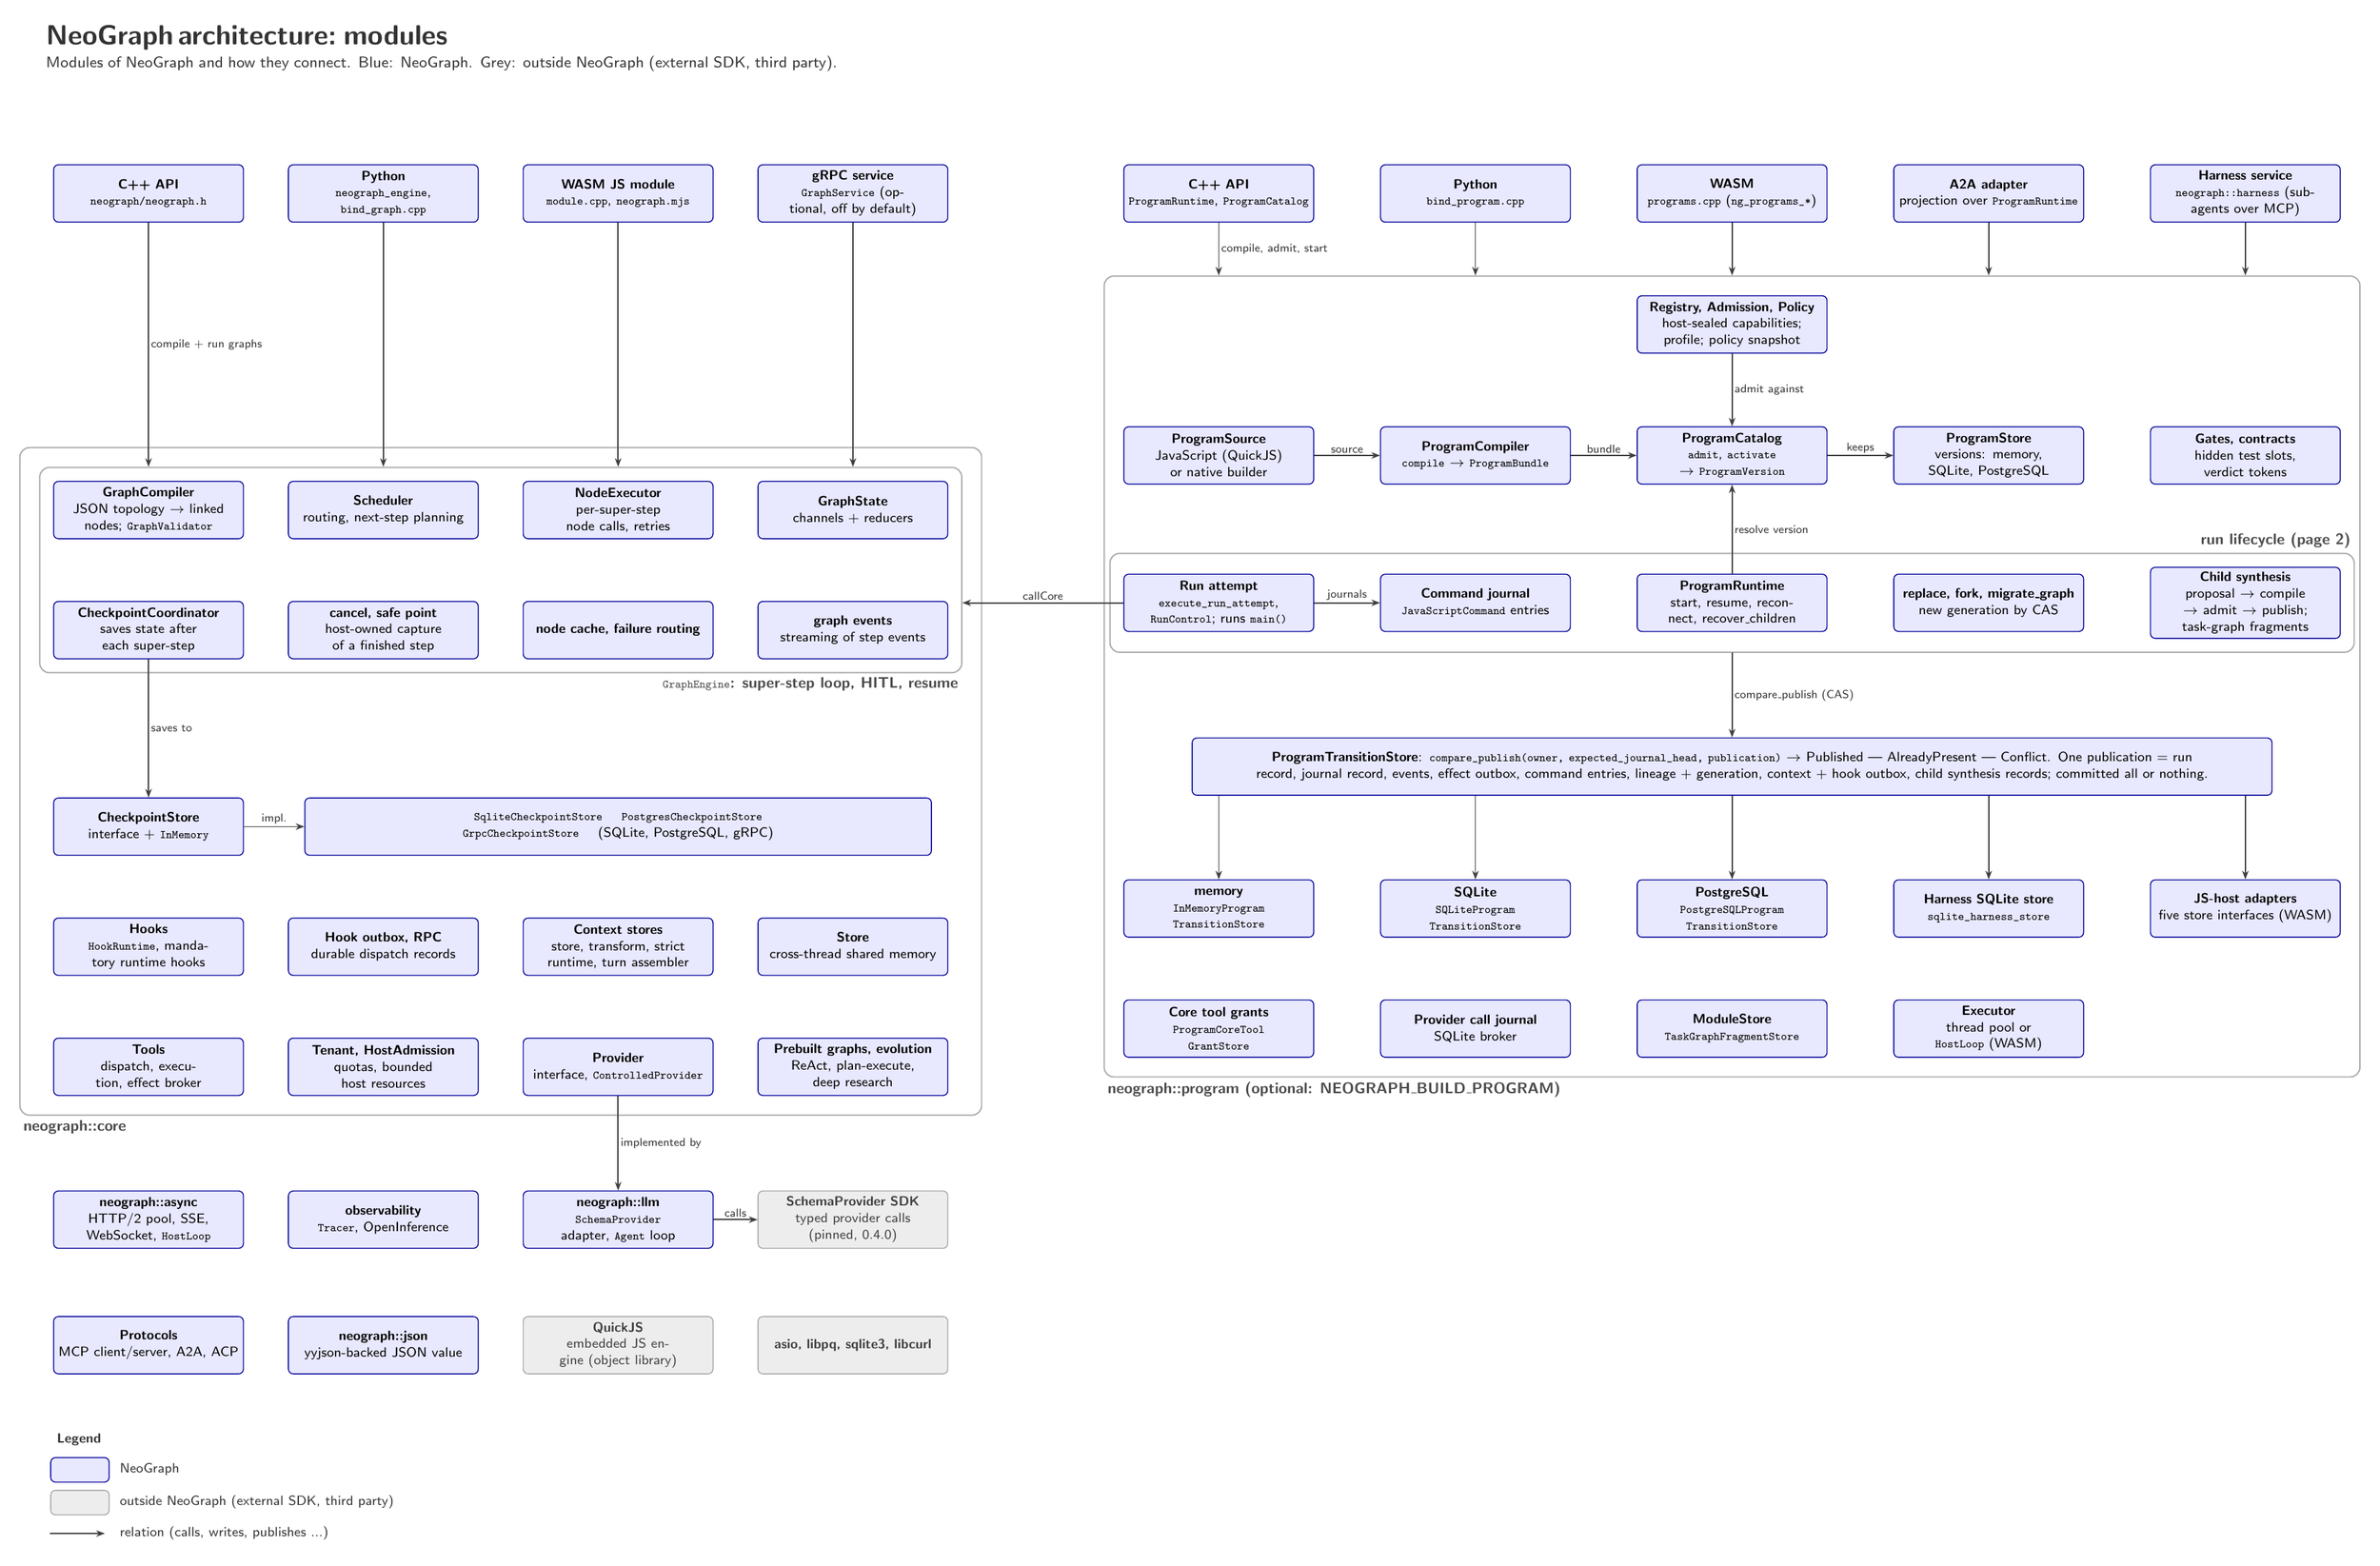
\begin{tikzpicture}[x=1cm,y=1cm]
\node[lab,anchor=north west,text width=40cm] at (0,37.4) {\textbf{\Large NeoGraph architecture: modules}\\[2pt]{\footnotesize Modules of NeoGraph and how they connect. Blue: NeoGraph. Grey: outside NeoGraph (external SDK, third party).}};
% source: include/neograph/neograph.h
\node[master] (g_cpp) at (2.0,34.2) {\textbf{C++ API}\\\cn{neograph/neograph.h}};
% source: bindings/python/src/bind_graph.cpp
\node[master] (g_py) at (6.3,34.2) {\textbf{Python}\\\cn{neograph_engine}, \cn{bind_graph.cpp}};
% source: wasm/module.cpp; wasm/neograph.mjs
\node[master] (g_wasm) at (10.6,34.2) {\textbf{WASM JS module}\\\cn{module.cpp}, \cn{neograph.mjs}};
% source: src/grpc/graph_service.cpp
\node[master] (g_grpc) at (14.899999999999999,34.2) {\textbf{gRPC service}\\\cn{GraphService} (optional, off by default)};
% source: include/neograph/program/runtime.h
\node[master] (h_cpp) at (21.6,34.2) {\textbf{C++ API}\\\cn{ProgramRuntime}, \cn{ProgramCatalog}};
% source: bindings/python/src/bind_program.cpp
\node[master] (h_py) at (26.3,34.2) {\textbf{Python}\\\cn{bind_program.cpp}};
% source: wasm/programs.cpp
\node[master] (h_wasm) at (31.0,34.2) {\textbf{WASM}\\\cn{programs.cpp} (\cn{ng_programs_*})};
% source: src/a2a/program_adapter.cpp
\node[master] (h_a2a) at (35.7,34.2) {\textbf{A2A adapter}\\projection over \cn{ProgramRuntime}};
% source: src/mcp/harness.cpp
\node[master] (h_harn) at (40.4,34.2) {\textbf{Harness service}\\\cn{neograph::harness} (subagents over MCP)};
% source: src/core/graph_compiler.cpp; src/core/graph_validator.cpp
\node[master] (c_comp) at (2.0,28.4) {\textbf{GraphCompiler}\\JSON topology $\to$ linked nodes; \cn{GraphValidator}};
% source: src/core/scheduler.cpp
\node[master] (c_sched) at (6.3,28.4) {\textbf{Scheduler}\\routing, next-step planning};
% source: src/core/graph_executor.cpp
\node[master] (c_exec) at (10.6,28.4) {\textbf{NodeExecutor}\\per-super-step node calls, retries};
% source: src/core/graph_state.cpp
\node[master] (c_state) at (14.899999999999999,28.4) {\textbf{GraphState}\\channels + reducers};
% source: src/core/graph_coordinator.cpp
\node[master] (c_coord) at (2.0,26.2) {\textbf{CheckpointCoordinator}\\saves state after each super-step};
% source: src/core/cancel.cpp; src/core/graph_safe_point.cpp
\node[master] (c_safe) at (6.3,26.2) {\textbf{cancel, safe point}\\host-owned capture of a finished step};
% source: src/core/node_cache.cpp; src/core/failure_routing.cpp
\node[master] (c_cache) at (10.6,26.2) {\textbf{node cache, failure routing}};
% source: src/core/graph_events.cpp
\node[master] (c_ev) at (14.899999999999999,26.2) {\textbf{graph events}\\streaming of step events};
% source: src/core/graph_engine.cpp
\node[frm,fit=(c_comp)(c_sched)(c_exec)(c_state)(c_coord)(c_safe)(c_cache)(c_ev)] (engframe) {};
\node[font=\sffamily\footnotesize\bfseries,text=black!70,anchor=north east,inner sep=2pt] at (engframe.south east) {\cn{GraphEngine}: super-step loop, HITL, resume};
% source: src/core/graph_checkpoint.cpp
\node[master] (c_cp) at (2.0,22.6) {\textbf{CheckpointStore}\\interface + \cn{InMemory}};
% source: src/core/sqlite_checkpoint.cpp; src/core/postgres_checkpoint.cpp; src/grpc/grpc_checkpoint.cpp
\node[master,text width=11.3cm] (c_cpi) at (10.6,22.6) {\cn{SqliteCheckpointStore} \quad \cn{PostgresCheckpointStore}\\\cn{GrpcCheckpointStore} \quad (SQLite, PostgreSQL, gRPC)};
% source: src/core/hook.cpp; src/core/hook_runtime.cpp
\node[master] (c_hook) at (2.0,20.4) {\textbf{Hooks}\\\cn{HookRuntime}, mandatory runtime hooks};
% source: src/core/hook_outbox.cpp; src/core/hook_rpc.cpp
\node[master] (c_hout) at (6.3,20.4) {\textbf{Hook outbox, RPC}\\durable dispatch records};
% source: src/core/context_store.cpp; src/core/context_transform.cpp; src/core/strict_runtime.cpp; src/core/runtime_turn_assembler.cpp
\node[master] (c_ctx) at (10.6,20.4) {\textbf{Context stores}\\store, transform, strict runtime, turn assembler};
% source: src/core/store.cpp
\node[master] (c_store) at (14.899999999999999,20.4) {\textbf{Store}\\cross-thread shared memory};
% source: src/core/tool_dispatch.cpp; src/core/tool_execution.cpp; src/core/sqlite_tool_effect_broker.cpp
\node[master] (c_tool) at (2.0,18.2) {\textbf{Tools}\\dispatch, execution, effect broker};
% source: src/core/tenant.cpp; src/core/host_admission.cpp
\node[master] (c_ten) at (6.3,18.2) {\textbf{Tenant, HostAdmission}\\quotas, bounded host resources};
% source: src/core/provider.cpp; src/core/controlled_provider.cpp
\node[master] (c_prov) at (10.6,18.2) {\textbf{Provider}\\interface, \cn{ControlledProvider}};
% source: src/core/react_graph.cpp; src/core/plan_execute_graph.cpp; src/core/deep_research_graph.cpp; src/core/evolution.cpp
\node[master] (c_pre) at (14.899999999999999,18.2) {\textbf{Prebuilt graphs, evolution}\\ReAct, plan-execute, deep research};
\node[frm,inner sep=10pt,fit=(engframe)(c_cp)(c_cpi)(c_hook)(c_hout)(c_ctx)(c_store)(c_tool)(c_ten)(c_prov)(c_pre)] (coreframe) {};
\node[font=\sffamily\footnotesize\bfseries,text=black!70,anchor=north west,inner sep=2pt] at (coreframe.south west) {neograph::core};
% source: src/program/registry.cpp; src/program/admission.cpp
\node[master] (p_pol) at (31.0,31.8) {\textbf{Registry, Admission, Policy}\\host-sealed capabilities; profile; policy snapshot};
% source: src/program/source.cpp; src/program/javascript.cpp; src/program/authoring.cpp
\node[master] (p_src) at (21.6,29.4) {\textbf{ProgramSource}\\JavaScript (QuickJS) or native builder};
% source: src/program/compiler.cpp; src/program/bundle.cpp
\node[master] (p_cmp) at (26.3,29.4) {\textbf{ProgramCompiler}\\\cn{compile} $\to$ \cn{ProgramBundle}};
% source: src/program/catalog.cpp; src/program/version.cpp; src/program/activation.cpp
\node[master] (p_cat) at (31.0,29.4) {\textbf{ProgramCatalog}\\\cn{admit}, \cn{activate} $\to$ \cn{ProgramVersion}};
% source: src/program/store.cpp; src/program/sqlite_store.cpp; src/program/postgres_store.cpp
\node[master] (p_ps) at (35.7,29.4) {\textbf{ProgramStore}\\versions: memory, SQLite, PostgreSQL};
% source: src/program/gate.cpp; src/program/contract.cpp
\node[master] (p_gate) at (40.4,29.4) {\textbf{Gates, contracts}\\hidden test slots, verdict tokens};
% source: src/program/run_attempt.cpp; src/program/run_control.h
\node[master] (p_att) at (21.6,26.7) {\textbf{Run attempt}\\\cn{execute_run_attempt}, \cn{RunControl}; runs \cn{main()}};
% source: src/program/command.cpp; src/program/command_journal.cpp
\node[master] (p_cmd) at (26.3,26.7) {\textbf{Command journal}\\\cn{JavaScriptCommand} entries};
% source: src/program/runtime.cpp
\node[master] (p_rt) at (31.0,26.7) {\textbf{ProgramRuntime}\\start, resume, reconnect, recover\_children};
% source: src/program/replacement.cpp; src/program/fork.cpp; src/program/graph_migration.cpp
\node[master] (p_mig) at (35.7,26.7) {\textbf{replace, fork, migrate\_graph}\\new generation by CAS};
% source: src/program/child_synthesis.cpp; src/program/synthesis.cpp; src/program/task_graph_fragment.cpp
\node[master] (p_syn) at (40.4,26.7) {\textbf{Child synthesis}\\proposal $\to$ compile $\to$ admit $\to$ publish; task-graph fragments};
\node[frm,fit=(p_att)(p_cmd)(p_rt)(p_mig)(p_syn)] (rtframe) {};
\node[font=\sffamily\footnotesize\bfseries,text=black!70,anchor=south east,inner sep=2pt] at (rtframe.north east) {run lifecycle (page 2)};
% source: include/neograph/program/transition_store.h; src/program/transition_store.cpp
\node[master,text width=19.6cm] (t_if) at (31.0,23.7) {\textbf{ProgramTransitionStore}: \cn{compare_publish(owner, expected_journal_head, publication)} $\to$ Published | AlreadyPresent | Conflict. One publication = run record, journal record, events, effect outbox, command entries, lineage + generation, context + hook outbox, child synthesis records; committed all or nothing.};
% source: src/program/transition_store.cpp
\node[master] (t_mem) at (21.6,21.1) {\textbf{memory}\\\cn{InMemoryProgram}\\\cn{TransitionStore}};
% source: src/program/sqlite_transition_store.cpp
\node[master] (t_sq) at (26.3,21.1) {\textbf{SQLite}\\\cn{SQLiteProgram}\\\cn{TransitionStore}};
% source: src/program/postgres_transition_store.cpp
\node[master] (t_pg) at (31.0,21.1) {\textbf{PostgreSQL}\\\cn{PostgreSQLProgram}\\\cn{TransitionStore}};
% source: src/mcp/sqlite_harness_store.cpp
\node[master] (t_hs) at (35.7,21.1) {\textbf{Harness SQLite store}\\\cn{sqlite_harness_store}};
% source: wasm/js_stores.cpp
\node[master] (t_js) at (40.4,21.1) {\textbf{JS-host adapters}\\five store interfaces (WASM)};
% source: src/program/core_tool_grant_store.cpp; src/program/sqlite_core_tool_grant_store.cpp
\node[master] (o_grant) at (21.6,18.9) {\textbf{Core tool grants}\\\cn{ProgramCoreTool}\\\cn{GrantStore}};
% source: src/program/sqlite_provider_call_broker.cpp
\node[master] (o_pcj) at (26.3,18.9) {\textbf{Provider call journal}\\SQLite broker};
% source: src/program/module.cpp; src/program/task_graph_fragment.cpp
\node[master] (o_mod) at (31.0,18.9) {\textbf{ModuleStore}\\\cn{TaskGraphFragmentStore}};
% source: src/core/host_loop.cpp; src/program/runtime.cpp
\node[master] (o_exec) at (35.7,18.9) {\textbf{Executor}\\thread pool or \cn{HostLoop} (WASM)};
% plan
% plan
% plan
\node[frm,inner sep=10pt,fit=(p_pol)(p_src)(p_gate)(t_if)(t_js)(o_exec)] (pframe) {};
\node[font=\sffamily\footnotesize\bfseries,text=black!70,anchor=north west,inner sep=2pt] at (pframe.south west) {neograph::program (optional: NEOGRAPH\_BUILD\_PROGRAM)};
% source: src/llm/schema_provider.cpp; src/llm/agent.cpp
\node[master] (i_llm) at (10.6,15.4) {\textbf{neograph::llm}\\\cn{SchemaProvider} adapter, \cn{Agent} loop};
% source: cmake/NeoGraphSchemaProvider.cmake
\node[ext] (i_sp) at (14.899999999999999,15.4) {\textbf{SchemaProvider SDK}\\typed provider calls (pinned, 0.4.0)};
% source: src/async/http_client.cpp; src/async/ws_client.cpp; src/async/sse_parser.cpp
\node[master] (i_async) at (2.0,15.4) {\textbf{neograph::async}\\HTTP/2 pool, SSE, WebSocket, \cn{HostLoop}};
% source: src/observability/openinference.cpp
\node[master] (i_obs) at (6.3,15.4) {\textbf{observability}\\\cn{Tracer}, OpenInference};
% source: src/mcp/client.cpp; src/mcp/server.cpp; src/a2a/server.cpp; src/acp/server.cpp
\node[master] (i_proto) at (2.0,13.1) {\textbf{Protocols}\\MCP client/server, A2A, ACP};
% source: include/neograph/json.h; src/core/json.cpp
\node[master] (i_json) at (6.3,13.1) {\textbf{neograph::json}\\yyjson-backed JSON value};
% source: CMakeLists.txt
\node[ext] (i_qjs) at (10.6,13.1) {\textbf{QuickJS}\\embedded JS engine (object library)};
% source: CMakeLists.txt
\node[ext] (i_dep) at (14.899999999999999,13.1) {\textbf{asio, libpq, sqlite3, libcurl}};
% plan
% plan
% plan
% plan
% rel: g_cpp builds and runs graphs on the engine
\draw[fl] (g_cpp.south) -- (g_cpp |- engframe.north) node[el,right,pos=0.5] {compile + run graphs};
% rel: g_py builds and runs graphs on the engine
\draw[fl] (g_py.south) -- (g_py |- engframe.north);
% rel: g_wasm builds and runs graphs on the engine
\draw[fl] (g_wasm.south) -- (g_wasm |- engframe.north);
% rel: g_grpc builds and runs graphs on the engine
\draw[fl] (g_grpc.south) -- (g_grpc |- engframe.north);
% rel: h_cpp drives ProgramRuntime
\draw[fl] (h_cpp.south) -- (h_cpp |- pframe.north) node[el,right,pos=0.5] {compile, admit, start};
% rel: h_py drives ProgramRuntime
\draw[fl] (h_py.south) -- (h_py |- pframe.north);
% rel: h_wasm drives ProgramRuntime
\draw[fl] (h_wasm.south) -- (h_wasm |- pframe.north);
% rel: h_a2a drives ProgramRuntime
\draw[fl] (h_a2a.south) -- (h_a2a |- pframe.north);
% rel: h_harn drives ProgramRuntime
\draw[fl] (h_harn.south) -- (h_harn |- pframe.north);
\draw[fl] (p_src.east) -- (p_cmp.west) node[el,above,pos=0.5] {source};
\draw[fl] (p_cmp.east) -- (p_cat.west) node[el,above,pos=0.5] {bundle};
\draw[fl] (p_pol.south) -- (p_cat.north) node[el,right,pos=0.5] {admit against};
\draw[fl] (p_cat.east) -- (p_ps.west) node[el,above,pos=0.5] {keeps};
\draw[fl] (p_rt.north) -- (p_cat.south) node[el,right,pos=0.5] {resolve version};
\draw[fl] (p_att.east) -- (p_cmd.west) node[el,above,pos=0.5] {journals};
\draw[fl] (p_att.west) -- (engframe.east |- p_att.west) node[el,above,pos=0.5] {callCore};
\draw[fl] (rtframe.south) -- (t_if.north |- rtframe.south) -- (t_if.north) node[el,right,pos=0.5] {compare\_publish (CAS)};
\draw[fl] (t_if.south -| t_mem.north) -- (t_mem.north);
\draw[fl] (t_if.south -| t_sq.north) -- (t_sq.north);
\draw[fl] (t_if.south -| t_pg.north) -- (t_pg.north);
\draw[fl] (t_if.south -| t_hs.north) -- (t_hs.north);
\draw[fl] (t_if.south -| t_js.north) -- (t_js.north);
\draw[fl] (c_coord.south) -- (c_cp.north) node[el,right,pos=0.5] {saves to};
\draw[fl] (c_prov.south) -- (i_llm.north) node[el,right,pos=0.5] {implemented by};
\draw[fl] (i_llm.east) -- (i_sp.west) node[el,above,pos=0.5] {calls};
\draw[fl] (c_cp.east) -- (c_cpi.west) node[el,above,pos=0.5] {impl.};
\node[lab,anchor=north west] at (0.2,11.6) {\textbf{Legend}};
\node[master,text width=1.0cm,minimum height=0.45cm,anchor=north west,inner sep=1pt] (lgmaster) at (0.2,11.05) {};
\node[lab,anchor=west] at (1.35,10.83) {NeoGraph};
\node[ext,text width=1.0cm,minimum height=0.45cm,anchor=north west,inner sep=1pt] (lgext) at (0.2,10.45) {};
\node[lab,anchor=west] at (1.35,10.23) {outside NeoGraph (external SDK, third party)};
\draw[fl] (0.2,9.65) -- (1.2,9.65);
\node[lab,anchor=west] at (1.35,9.65) {relation (calls, writes, publishes ...)};
\end{tikzpicture}

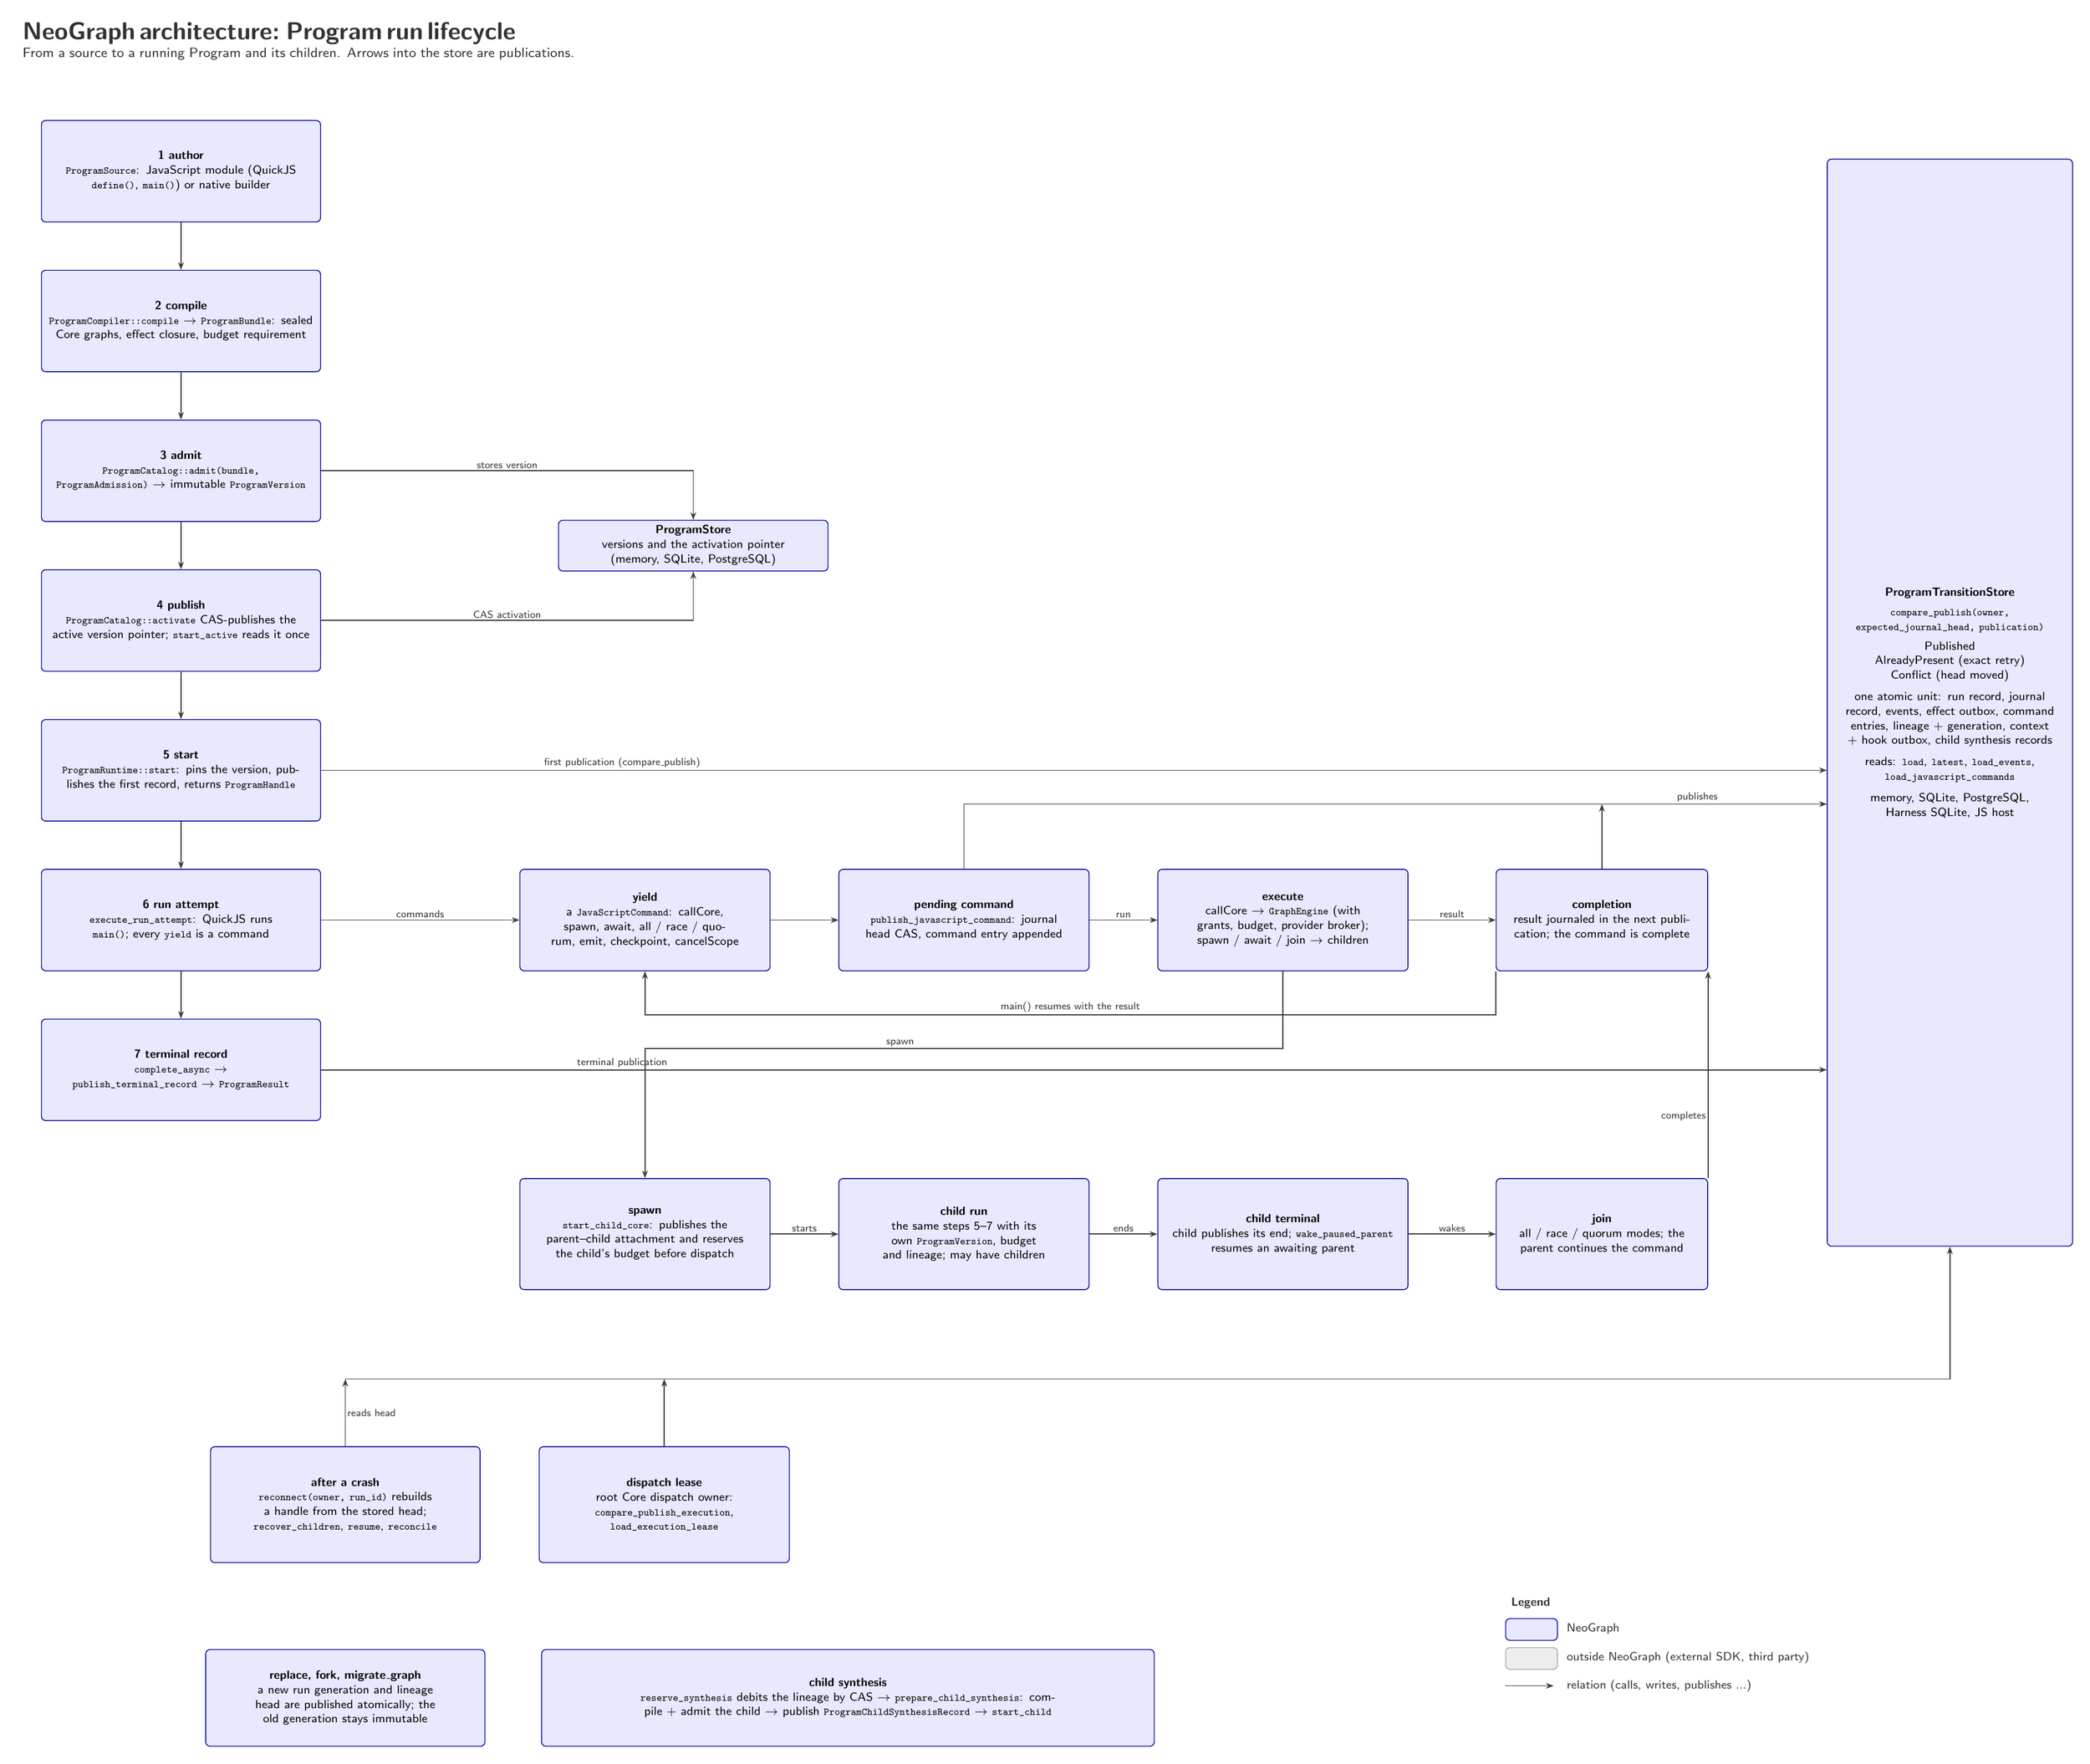
\begin{tikzpicture}[x=1cm,y=1cm]
\node[lab,anchor=north west,text width=40cm] at (0,36.2) {\textbf{\Large NeoGraph architecture: Program run lifecycle}\\[2pt]{\footnotesize From a source to a running Program and its children. Arrows into the store are publications. }};
% source: src/program/source.cpp; src/program/authoring.cpp
\node[master,text width=5.6cm,minimum height=2.1cm] (s1) at (3.4,33.0) {\textbf{1 author}\\\cn{ProgramSource}: JavaScript module (QuickJS \cn{define()}, \cn{main()}) or native builder};
% source: src/program/compiler.cpp; src/program/bundle.cpp
\node[master,text width=5.6cm,minimum height=2.1cm] (s2) at (3.4,29.9) {\textbf{2 compile}\\\cn{ProgramCompiler::compile} $\to$ \cn{ProgramBundle}: sealed Core graphs, effect closure, budget requirement};
% source: src/program/catalog.cpp; src/program/version.cpp
\node[master,text width=5.6cm,minimum height=2.1cm] (s3) at (3.4,26.8) {\textbf{3 admit}\\\cn{ProgramCatalog::admit(bundle, ProgramAdmission)} $\to$ immutable \cn{ProgramVersion}};
% source: src/program/activation.cpp; include/neograph/program/catalog.h
\node[master,text width=5.6cm,minimum height=2.1cm] (s4) at (3.4,23.7) {\textbf{4 publish}\\\cn{ProgramCatalog::activate} CAS-publishes the active version pointer; \cn{start_active} reads it once};
% source: src/program/runtime.cpp
\node[master,text width=5.6cm,minimum height=2.1cm] (s5) at (3.4,20.6) {\textbf{5 start}\\\cn{ProgramRuntime::start}: pins the version, publishes the first record, returns \cn{ProgramHandle}};
% source: src/program/run_attempt.cpp
\node[master,text width=5.6cm,minimum height=2.1cm] (s6) at (3.4,17.5) {\textbf{6 run attempt}\\\cn{execute_run_attempt}: QuickJS runs \cn{main()}; every \cn{yield} is a command};
% source: src/program/runtime.cpp; src/program/result.cpp
\node[master,text width=5.6cm,minimum height=2.1cm] (s7) at (3.4,14.4) {\textbf{7 terminal record}\\\cn{complete_async} $\to$ \cn{publish_terminal_record} $\to$ \cn{ProgramResult}};
\draw[fl] (s1.south) -- (s2.north);
\draw[fl] (s2.south) -- (s3.north);
\draw[fl] (s3.south) -- (s4.north);
\draw[fl] (s4.south) -- (s5.north);
\draw[fl] (s5.south) -- (s6.north);
\draw[fl] (s6.south) -- (s7.north);
% source: src/program/store.cpp; src/program/sqlite_store.cpp; src/program/postgres_store.cpp
\node[master,text width=5.4cm] (ps) at (14.0,25.25) {\textbf{ProgramStore}\\versions and the activation pointer (memory, SQLite, PostgreSQL)};
\draw[fl] (s3.east) -| (ps.north) node[el,above,pos=0.25] {stores version};
\draw[fl] (s4.east) -| (ps.south) node[el,above,pos=0.25] {CAS activation};
% source: include/neograph/program/transition_store.h; src/program/transition_store.cpp
\node[master,text width=4.9cm,minimum height=22.5cm] (bar) at (40.0,22.0) {\textbf{ProgramTransitionStore}\\[3pt]\cn{compare_publish(owner, expected_journal_head, publication)}\\[3pt]Published\\AlreadyPresent (exact retry)\\Conflict (head moved)\\[4pt]one atomic unit: run record, journal record, events, effect outbox, command entries, lineage + generation, context + hook outbox, child synthesis records\\[4pt]reads: \cn{load}, \cn{latest}, \cn{load_events}, \cn{load_javascript_commands}\\[4pt]memory, SQLite, PostgreSQL, Harness SQLite, JS host};
% source: src/program/command.cpp
\node[master,text width=5.0cm,minimum height=2.1cm] (k1) at (13.0,17.5) {\textbf{yield}\\a \cn{JavaScriptCommand}: callCore, spawn, await, all / race / quorum, emit, checkpoint, cancelScope};
% source: src/program/command_journal.cpp; src/program/run_attempt.cpp
\node[master,text width=5.0cm,minimum height=2.1cm] (k2) at (19.6,17.5) {\textbf{pending command}\\\cn{publish_javascript_command}: journal head CAS, command entry appended};
% source: src/program/run_attempt.cpp; src/program/catalog.cpp
\node[master,text width=5.0cm,minimum height=2.1cm] (k3) at (26.2,17.5) {\textbf{execute}\\callCore $\to$ \cn{GraphEngine} (with grants, budget, provider broker); spawn / await / join $\to$ children};
% source: src/program/command_journal.cpp
\node[master,text width=4.2cm,minimum height=2.1cm] (k4) at (32.8,17.5) {\textbf{completion}\\result journaled in the next publication; the command is complete};
\draw[fl] (s6.east) -- (k1.west) node[el,above,pos=0.5] {commands};
\draw[fl] (k1.east) -- (k2.west);
\draw[fl] (k2.east) -- (k3.west) node[el,above,pos=0.5] {run};
\draw[fl] (k3.east) -- (k4.west) node[el,above,pos=0.5] {result};
\draw[fl] (k4.south west) -- ++(0,-0.9) -| (k1.south) node[el,above,pos=0.25] {main() resumes with the result};
\draw[fl] (k2.north) -- (k2.north |- 0,19.9) -- (bar.west |- 0,19.9) node[el,above,pos=0.85] {publishes};
\draw[fl] (k4.north) -- (k4.north |- 0,19.9);
\draw[fl] (s5.east) -- (bar.west |- s5.east) node[el,above,pos=0.2] {first publication (compare\_publish)};
\draw[fl] (s7.east) -- (bar.west |- s7.east) node[el,above,pos=0.2] {terminal publication};
% source: src/program/runtime.cpp; include/neograph/program/run_record.h
\node[master,text width=5.0cm,minimum height=2.3cm] (c1) at (13.0,11.0) {\textbf{spawn}\\\cn{start_child_core}: publishes the parent--child attachment and reserves the child's budget before dispatch};
% source: src/program/runtime.cpp
\node[master,text width=5.0cm,minimum height=2.3cm] (c2) at (19.6,11.0) {\textbf{child run}\\the same steps 5--7 with its own \cn{ProgramVersion}, budget and lineage; may have children};
% source: src/program/run_attempt.cpp; src/program/run_control.h
\node[master,text width=5.0cm,minimum height=2.3cm] (c3) at (26.2,11.0) {\textbf{child terminal}\\child publishes its end; \cn{wake_paused_parent} resumes an awaiting parent};
% source: src/program/run_attempt.cpp
\node[master,text width=4.2cm,minimum height=2.3cm] (c4) at (32.8,11.0) {\textbf{join}\\all / race / quorum modes; the parent continues the command};
\draw[fl] (k3.south) -- ++(0,-1.6) -| (c1.north) node[el,above,pos=0.3] {spawn};
\draw[fl] (c1.east) -- (c2.west) node[el,above,pos=0.5] {starts};
\draw[fl] (c2.east) -- (c3.west) node[el,above,pos=0.5] {ends};
\draw[fl] (c3.east) -- (c4.west) node[el,above,pos=0.5] {wakes};
\draw[fl] (c4.north east) -- (k4.south east) node[el,left,pos=0.3] {completes};
% source: include/neograph/program/runtime.h
\node[master,text width=5.4cm,minimum height=2.4cm] (r1) at (6.8,5.4) {\textbf{after a crash}\\\cn{reconnect(owner, run_id)} rebuilds a handle from the stored head; \cn{recover_children}, \cn{resume}, \cn{reconcile}};
% source: include/neograph/program/transition_store.h
\node[master,text width=5.0cm,minimum height=2.4cm] (r2) at (13.4,5.4) {\textbf{dispatch lease}\\root Core dispatch owner: \cn{compare_publish_execution}, \cn{load_execution_lease}};
% plan
\draw[fl] (r1.north) -- (r1.north |- 0,8.0) node[el,right,pos=0.5] {reads head};
\draw[fl] (r2.north) -- (r2.north |- 0,8.0);
\draw[fl] (r1.north |- 0,8.0) -- (bar.south |- 0,8.0) -- (bar.south);
% source: src/program/replacement.cpp; src/program/fork.cpp; src/program/graph_migration.cpp; src/program/lineage.cpp
\node[master,text width=5.6cm,minimum height=2.0cm] (y1) at (6.8,1.4) {\textbf{replace, fork, migrate\_graph}\\a new run generation and lineage head are published atomically; the old generation stays immutable};
% source: include/neograph/program/runtime.h; src/program/child_synthesis.cpp; src/program/synthesis.cpp; include/neograph/program/module.h
\node[master,text width=12.5cm,minimum height=2.0cm] (y2) at (17.2,1.4) {\textbf{child synthesis}\\\cn{reserve_synthesis} debits the lineage by CAS $\to$ \cn{prepare_child_synthesis}: compile + admit the child $\to$ publish \cn{ProgramChildSynthesisRecord} $\to$ \cn{start_child}};
% plan
\node[lab,anchor=north west] at (30.8,3.6) {\textbf{Legend}};
\node[master,text width=1.0cm,minimum height=0.45cm,anchor=north west,inner sep=1pt] (lgmaster) at (30.8,3.05) {};
\node[lab,anchor=west] at (31.95,2.83) {NeoGraph};
\node[ext,text width=1.0cm,minimum height=0.45cm,anchor=north west,inner sep=1pt] (lgext) at (30.8,2.45) {};
\node[lab,anchor=west] at (31.95,2.23) {outside NeoGraph (external SDK, third party)};
\draw[fl] (30.8,1.65) -- (31.8,1.65);
\node[lab,anchor=west] at (31.95,1.65) {relation (calls, writes, publishes ...)};
\end{tikzpicture}
\end{document}
